\documentclass[12pt]{article}

% \usepackage{framed}
% \usepackage{url}
% \usepackage{ifthen}
% \usepackage{longtable}
% \usepackage{fancyvrb}
% \usepackage{cancel}

% \usepackage{lmodern}
\usepackage{amsmath,amssymb,gensymb}%,amsthm,amsfonts,,amscd}
\usepackage[arrowdel]{physics} 
% \usepackage{multirow,booktabs}
\usepackage[dvipsnames,table]{xcolor}
% \usepackage{fullpage}
% \usepackage{lastpage}
\usepackage{pstricks} 
\usepackage{graphicx}
\graphicspath{{../figures/}}
\definecolor{mygreen}{RGB}{28,172,0}
\definecolor{mylilas}{RGB}{170,55,241}
\definecolor{deepblue}{rgb}{0,0,0.5}
\definecolor{deepred}{rgb}{0.6,0,0}
\definecolor{deepgreen}{rgb}{0,0.5,0}

\usepackage{fancyhdr}
% \usepackage{mathrsfs}
% \usepackage{wrapfig}
% \usepackage{setspace}
% \usepackage{calc}
\usepackage{multicol}
\usepackage{listings}



% \usepackage{siunitx}

% \usepackage{cancel}
% %\usepackage[retainorgcmds]{IEEEtrantools}
% \usepackage[margin=3cm]{geometry}
% \newlength{\tabcont}
% \setlength{\parindent}{0.0in}
% \setlength{\parskip}{0.05in}
% \usepackage{empheq}
% \usepackage{framed}
% \usepackage{mdframed}
\usepackage{systeme}

\usepackage{tcolorbox}
% \usepackage{chemfig,chemmacros,chemnum}
% \usepackage{chemformula}

% \usepackage{tcolorbox}
\usepackage{url}
   \let\oldurl\url
\usepackage{hyperref}
   \let\linkurl\url
   \let\url\oldurl


% \RequirePackage{setspace}
% \RequirePackage{lastpage}
% \RequirePackage{extramarks}
% \RequirePackage{chngpage}
% \RequirePackage{soul}


\usepackage{makecell}
\usepackage{caption}
% \usepackage{fancybox}

% %\RequirePackage[text]{amsthm}
% %\RequirePackage{array}
% %\RequirePackage{amscd}
% %\RequirePackage{array}\RequirePackage{dcolumn}
% %\putfig{3.5truein}{PSfig1.3}{Peter's winnings in 40 plays of heads or tails.}{fig 1.3}

% \newcommand{\dx}{\, dx}
% \newcommand{\dy}{\, dy}
% \newcommand{\dt}{\, dt}
% \newcommand{\dth}{\, d\theta}
% \newcommand{\dr}{\, dr}
% \newcommand{\du}{\, du}
\newcommand\uvec[1]{\textbf{#1}}
% \newcommand{\iu}{\hat{\uvec{i}}}
% \newcommand{\ju}{\hat{\uvec{j}}}
% \newcommand{\ku}{\hat{\uvec{k}}}

% \newcommand{\emx}[1]{{\em{#1}\/}}
% \newcommand{\abin}{{\it ab initio}}
% \newcommand{\bs}{\boldsymbol}
% \newcommand{\citenum}{\cite}
% \newcommand{\dGo}{\ensuremath{\Delta G_0}}
% \newcommand{\dG}[2]{\ensuremath{\Delta G_{\rm #1}^{\rm #2}}}
% \newcommand{\dX}[3]{\ensuremath{\Delta #1_{\rm #2}^{\rm #3}}}
% \newcommand{\ddgo}[1]{\ensuremath{\Delta \Delta G_{\rm solv}^{\rm #1}}}
% \newcommand{\ddgstarcat}{\ensuremath{\Delta \Delta g^{\ddagger}_{\rm cat}}}
% \newcommand{\ddgstar}{\ensuremath{\Delta \dgstar}}
% \newcommand{\ddgt}[2]{\ensuremath{\Delta \Delta G_{\rm solv}^{\rm #1, \rm #2}}}
% \newcommand{\ddsstarprime}{\ensuremath{(\Delta \dsstar)'}}
% \newcommand{\deltaepsel}{\ensuremath{\Delta \varepsilon_{\rm el}}}
% \newcommand{\deltaeps}{\ensuremath{\Delta \varepsilon}}
% \newcommand{\dgab}[2]{\ensuremath{\Delta g_{\rm #1}^{\rm #2}}}
% \newcommand{\dga}[1]{\ensuremath{\Delta g_{\rm #1}}}
% \newcommand{\dgb}[1]{\ensuremath{\Delta g^{\rm #1}}}
% \newcommand{\dgcage}{\ensuremath{\Delta g_{\rm cage}}}
% \newcommand{\dgcat}{\ensuremath{\Delta g_{\rm cat}}}
% \newcommand{\dgsoltsatsa}{\ensuremath{\dgsol (\rm TSA)_{\rm TSA}}}
% \newcommand{\dgsoltstsa}{\ensuremath{\dgsol (\rm TS)_{\rm TSA}}}
% \newcommand{\dgsoltsts}{\ensuremath{\dgsol (\rm TS)_{\rm TS}}}
% \newcommand{\dgsol}{\ensuremath{\Delta G_{\rm sol}}}
% \newcommand{\dgstarcage}{\ensuremath{\dgstar_{\rm cage}}}
% \newcommand{\dgstarcat}{\ensuremath{\dgstar_{\rm cat}}}
% \newcommand{\dgstarw}{\ensuremath{\dgstar_{\rm w}}}
% \newcommand{\dgstar}{\ensuremath{\Delta g^{\ddagger}}}
% \newcommand{\dgw}{\ensuremath{\Delta g_{\rm w}}}
% \newcommand{\dg}[2]{\ensuremath{\Delta g_{\rm #1}^{\rm #2}}}
% \newcommand{\dino}{\texttt{DINO}}
% \newcommand{\dsstarcageprime}{\ensuremath{(\dsstarcage)'}}
% \newcommand{\dsstarcage}{\ensuremath{\dsstar_{\rm cage}}}
% \newcommand{\dsstarcatprime}{\ensuremath{(\dsstarcat)'}}
% \newcommand{\dsstarcat}{\ensuremath{\dsstar_{\rm cat}}}
% \newcommand{\dsstarwprime}{\ensuremath{(\dsstarw)'}}
% \newcommand{\dsstarw}{\ensuremath{\dsstar_{\rm w}}}
% \newcommand{\dsstar}{\ensuremath{\Delta S^{\ddagger}}}
% \newcommand{\eg}{{\it e.g.}}
% \newcommand{\etal}{{\it et al.}}
% \newcommand{\gamess}{\texttt{GAMESS}}
% \newcommand{\gauss}{\texttt{GAUSSIAN} 98}
% \newcommand{\golpe}{\texttt{GOLPE}}
% \newcommand{\grid}{\texttt{GRID}}
% \newcommand{\ie}{{\it i.e.}}
% \newcommand{\ith}{{\it i}$^{\rm th}$\ }
% \newcommand{\kbt}{\ensuremath{k_{\rm B} T}}
% \newcommand{\kb}{\ensuremath{k_{\rm B}}}
% \newcommand{\kcage}{\ensuremath{k_{\rm cage}}}
% \newcommand{\kcatkm}{\ensuremath{k_{\rm cat}/K_{\rm M}}}
% \newcommand{\kcat}{\ensuremath{k_{\rm cat}}}
% \newcommand{\km}{kcal mol$^-1$}
% \newcommand{\knon}{\ensuremath{k_{\rm non}}}
% \newcommand{\kw}{\ensuremath{k_{\rm w}}}
% \newcommand{\mepsim}{\texttt{MEPSIM}}
% \newcommand{\mgp}[1]{\marginpar{\scriptsize{#1}}}
% \newcommand{\mipsim}{\texttt{MIPSIM}}
% \newcommand{\mola}{\texttt{MOLARIS}}
% \newcommand{\msms}{\texttt{MSMS}}
% \newcommand{\pdras}{p21$^{\rm ras}$}
% \newcommand{\rgran}{\ensuremath{\mathbb{R}}}
% \newcommand{\rx}[2]{\ensuremath{#1_{\rm #2}}}
% \newcommand{\vs}{{\it vs.}}
% \newcommand{\z}[1]{\ensuremath{\mathbf{#1}}}
% \newcommand{\composed}[2]{#1\mathbin\circ #2}
% \newcommand{\wrt}[1]{{\mbox{\scriptsize w.r.t. \( #1 \)} }}
% \newcommand{\polyspace}{\mathcal{P}}
% \newcommand{\matspace}{\mathcal{M}}
% %\newcommand{\C}{\mathbb{C}}
% \newcommand{\N}{\mathbb{N}}
% \newcommand{\Q}{\mathbb{Q}}
% \newcommand{\Z}{\mathbb{Z}}
% \renewcommand{\Re}{\mathbb{R}}
% \newcommand{\rtres}{\ensuremath{\Re^3}}
% \newcommand{\union}{\cup}
% \newcommand{\dotprod}{\cdot}
% \newcommand*\pkg[1]{\textsf{#1}}

% \newcommand{\trans}[1]{{#1}^{\ensuremath{\mathsf{T}}}} % transpose
% \newcommand{\nbyn}[1]{\ensuremath{#1 \! \times \! #1 }}
% \newcommand{\nbym}[2]{#1 \! \times \! #2 }       % Use in math mode.
% \newcommand{\cat}[2]{#1\!\mathbin{\raise.6ex\hbox{\( {}^\frown \)}}\!#2}
% \newcommand{\generalmatrix}[3]{ %arg1: low-case letter, arg2: rows, arg3: cols
%                \left(
%                   \begin{array}{cccc}
%                     #1_{1,1}  &#1_{1,2}  &\ldots  &#1_{1,#2}  \\
%                     #1_{2,1}  &#1_{2,2}  &\ldots  &#1_{2,#2}  \\
%                               &\vdots                         \\
%                     #1_{#3,1} &#1_{#3,2} &\ldots  &#1_{#3,#2}
%                   \end{array}
%                \right)  }
% \newcommand{\colvec}[1]{\begin{pmatrix} #1 \end{pmatrix}}
% \newcommand{\pr}[1]{\ensuremath{\mathrm{Pr}(#1)}}
% \newcommand{\rep}[2]{ {\rm Rep}_{#2}(#1) }
% \newcommand{\mapsunder}[1]{\stackrel{#1}{\longmapsto}}
% \newcommand{\map}[3]{\mbox{$#1\colon #2\to #3$}}
% \newcommand{\identity}{\mbox{id}}
% \newcommand{\stdbasis}{{\cal E}}
% \newcommand{\sequence}[1]{ \langle#1\rangle }
% \newcommand{\spacer}{\rule[-3mm]{0mm}{8mm}}
% \newcommand{\email}[1]{\url{#1}}
% \newcommand{\zero}{\vec{0}}
% \newcommand{\proj}[2]{\mbox{proj}_{#2}({#1}) }
% %\AtBeginDocument{\newlength{\heightofcdot}
% %\newlength{\widthofcdot}
% %\settoheight{\heightofcdot}{$\cdot$}
% %\settowidth{\widthofcdot}{$\cdot$}
% %\newsavebox{\dotprodcircle}
% %\savebox{\dotprodcircle}{\includegraphics{dotprod.1}}
% %\newcommand{\dotprod}{\mathbin{\raisebox{.5\heightofcdot}{%
% %          \makebox[\widthofcdot]{$\smash{\usebox{\dotprodcircle}}$}}}}}
% \newcommand{\spanof}[1]{\relax [#1\relax ]} % no optional argument!
% \newcommand{\set}[1]{\mbox{$\{#1\}$}} \newcommand{\suchthat}{\bigm|}
% \newcommand{\deter}[1]{ \mathchoice{\left|#1\right|}{|#1|}{|#1|}{|#1|} }
% \newcommand{\secuence}[1]{ \langle#1\rangle }
% \newcommand{\basis}[2]{\secuence{\vec{#1}_1,\ldots,\vec{#1}_{#2}}}



% %--------linsys
% %  Use as \begin{linsys}{3}
% %           x &+ &3y &+ &a &= &7 \\
% %           x &- &3y &+ &a &= &7
% %         \end{linsys}
% % Remark: TeXbook pp. 167-170 says to put a medmuskip around a +; and that's
% % 4/18-ths of an em.  Why does 2/18-ths of an em work?  I don't know, but
% % comparing to a regular displayed equation suggests it is right.
% % (darseneau says LaTeX puts in half an \arraycolsep.)
% \newenvironment{linsys}[2][m]{%
% \setlength{\arraycolsep}{.1111em} % p. 170 TeXbook; a medmuskip
% \begin{array}[#1]{@{}*{#2}{rc}r@{}}
% }{%
% \end{array}}


% header and footer
\pagestyle{fancy}       %                %
\cfoot{
\includegraphics[width=2cm]{FCTE}}                %
\rfoot{\thepage}        %
\renewcommand\headrulewidth{0.4pt}   %
\renewcommand\footrulewidth{0.4pt}   %

\usepackage[lastexercise]{exercise}

%numeracions dels llistats
\usepackage{enumitem}
\newlist{llista}{enumerate}{3}
\setlist[llista,1]{label=(\arabic*)}
\setlist[llista,2]{label=(\arabic{llistai}.\arabic*)}
\setlist[llista,3]{label=(\arabic{llistai}.\arabic{llistaii}.\arabic*)}

%%%%%%%%%%%%%%%%%%%%%%%%%%%%%%%%%%%%%%%%%%%%%%
%%%%%%%%%%%%%%%%%%%%%%%%%%%%%%%%%%%%%%%%%%%%%%

% comanda per definir Gauss-Jordan Elimination
\allowdisplaybreaks
\makeatletter
\newcounter{elimination@steps}
\newcolumntype{R}[1]{>{\raggedleft\arraybackslash$}p{#1}<{$}}
\def\elimination@num@rights{}
\def\elimination@num@variables{}
\def\elimination@col@width{}
\newenvironment{elimination}[4][0]
{
    \setcounter{elimination@steps}{0}
    \def\elimination@num@rights{#1}
    \def\elimination@num@variables{#2}
    \def\elimination@col@width{#3}
    \renewcommand{\arraystretch}{#4}
    \start@align\@ne\st@rredtrue\m@ne
}
{
    \endalign
    \ignorespacesafterend
}
\newcommand{\eliminationstep}[2]
{
    \ifnum\value{elimination@steps}>0\sim\quad\fi
    \left[
        \ifnum\elimination@num@rights>0
            \begin{array}
            {@{}*{\elimination@num@variables}{R{\elimination@col@width}}
            |@{}*{\elimination@num@rights}{R{\elimination@col@width}}}
        \else
            \begin{array}
            {@{}*{\elimination@num@variables}{R{\elimination@col@width}}}
        \fi
            #1
        \end{array}
    \right]
    &
    \begin{array}{l}
        #2
    \end{array}
    &%                                    moved second & here
    \addtocounter{elimination@steps}{1}
}
\makeatother

%%%%%%%%%%%%%%%%%%%%%%%%%%%%%%%%%%%%%%%%%%%%%%
%%%%%%%%%%%%%%%%%%%%%%%%%%%%%%%%%%%%%%%%%%%%%%

\usepackage{tikz}
\usepackage{tkz-graph}
\usepackage{pgfplots}
\usepackage{tkz-euclide}
\usetikzlibrary{patterns}
\usetikzlibrary{arrows,automata}
\usetikzlibrary{positioning,calc}%,quotes}
\usetikzlibrary{babel} % solve some problems with different languages like spanish
% Default fixed font does not support bold face
\DeclareFixedFont{\ttb}{T1}{txtt}{bx}{n}{12} % for bold
\DeclareFixedFont{\ttm}{T1}{txtt}{m}{n}{12}  % for normal

% Custom colors
\definecolor{deepblue}{rgb}{0,0,0.5}
\definecolor{deepred}{rgb}{0.6,0,0}
\definecolor{deepgreen}{rgb}{0,0.5,0}

\usepackage{listings}

\lstset{language=Matlab,%
    %basicstyle=\color{red},
    breaklines=true,%
    morekeywords={matlab2tikz},
    keywordstyle=\color{blue},%
    morekeywords=[2]{1}, keywordstyle=[2]{\color{black}},
    identifierstyle=\color{black},%
    stringstyle=\color{mylilas},
    commentstyle=\color{mygreen},%
    showstringspaces=false,%without this there will be a symbol in the places where there is a space
    numbers=left,%
    numberstyle={\tiny \color{black}},% size of the numbers
    numbersep=9pt, % this defines how far the numbers are from the text
    emph=[1]{for,end,break},emphstyle=[1]\color{red}, %some words to emphasise
    %emph=[2]{word1,word2}, emphstyle=[2]{style},
}

% Python style for highlighting
\newcommand\pythonstyle{\lstset{
language=Python,
basicstyle=\ttm,
morekeywords={self},              % Add keywords here
keywordstyle=\ttb\color{deepblue},
emph={MyClass,__init__},          % Custom highlighting
emphstyle=\ttb\color{deepred},    % Custom highlighting style
stringstyle=\color{deepgreen},
frame=tb,                         % Any extra options here
showstringspaces=false
}}


% Python environment
\lstnewenvironment{python}[1][]
{
\pythonstyle
\lstset{#1}
}
{}

% Python for external files
\newcommand\pythonexternal[2][]{{
\pythonstyle
\lstinputlisting[#1]{#2}}}

% Python for inline
\newcommand\pythoninline[1]{{\pythonstyle\lstinline!#1!}}

% \lstdefinestyle{mystyle}{%
%   numbers=left,
%   numberstyle=\small,
%   numbersep=8pt,
%   %language=Matlab,
%   style=Matlab-editor,
%   basicstyle=\ttfamily\small,
%   numbersep=25pt,
%   frame=none
% }

% rename lstlistings caption titles
\renewcommand\lstlistingname{Code}
\renewcommand\lstlistlistingname{Codes}
\def\lstlistingautorefname{Code}
\begin{document}



\title{Solved Exercises \\ \large Optimization and Operations Research \newline \newline 
\includegraphics[width = 60mm]{FCTE}
\author{Jordi Villà-Freixa}
\thanks{e.mail: \texttt{jordi.villa@uvic.cat}}}

\date{Last update: \today}
\maketitle
\tableofcontents
\listofexercises
\newpage

\begin{ExerciseList}
\section{Non-linear optimization}

\subsection{NLO with constraints}
\Exercise[label={ex:NLO2},title={coses}] 
A company wants to maximize its profit function given by:

\[
f(x, y) = -x^2 + 4xy - 2y^2
\]

where \(x\) and \(y\) represent the amount of resources allocated to two different projects.

The problem is subject to the following constraints:
\begin{enumerate}
    \item The total resources used must not exceed 30 units:
    \[
    x + 2y \leq 30
    \]
    \item The product of the resources allocated must be at least 50 units:
    \[
    xy \geq 50
    \]
    \item The relationship between the resource allocations must satisfy the following nonlinear constraint:
    \[
    y \leq \frac{3x^2}{100} + 5
    \]
\end{enumerate}

The company wants to find the values of \(x\) and \(y\) that maximize the profit \(f(x, y)\) under these constraints. 

Can you help the company drawing the problem in a graph? Can you identify the feasible region? Is the region convex?


\Answer 

This is \autoref{ex:NLO2}.

A company wants to maximize its profit function given by:

\[
f(x, y) = -x^2 + 4xy - 2y^2
\]

where \(x\) and \(y\) represent the amount of resources allocated to two different projects.

The problem is subject to the following constraints:
\begin{enumerate}
    \item The total resources used must not exceed 30 units:
    \[
    x + 2y \leq 30
    \]
    \item The product of the resources allocated must be at least 50 units:
    \[
    xy \geq 50
    \]
    \item The relationship between the resource allocations must satisfy the following nonlinear constraint:
    \[
    y \leq \frac{3x^2}{100} + 5
    \]
\end{enumerate}


Find the values of \(x\) and \(y\) that maximize the profit \(f(x, y)\) under these constraints.


The problem is shown in Figure \ref{Fig:NLO2}.

\begin{minipage}[t]{\linewidth}
  \vspace{-2ex}
        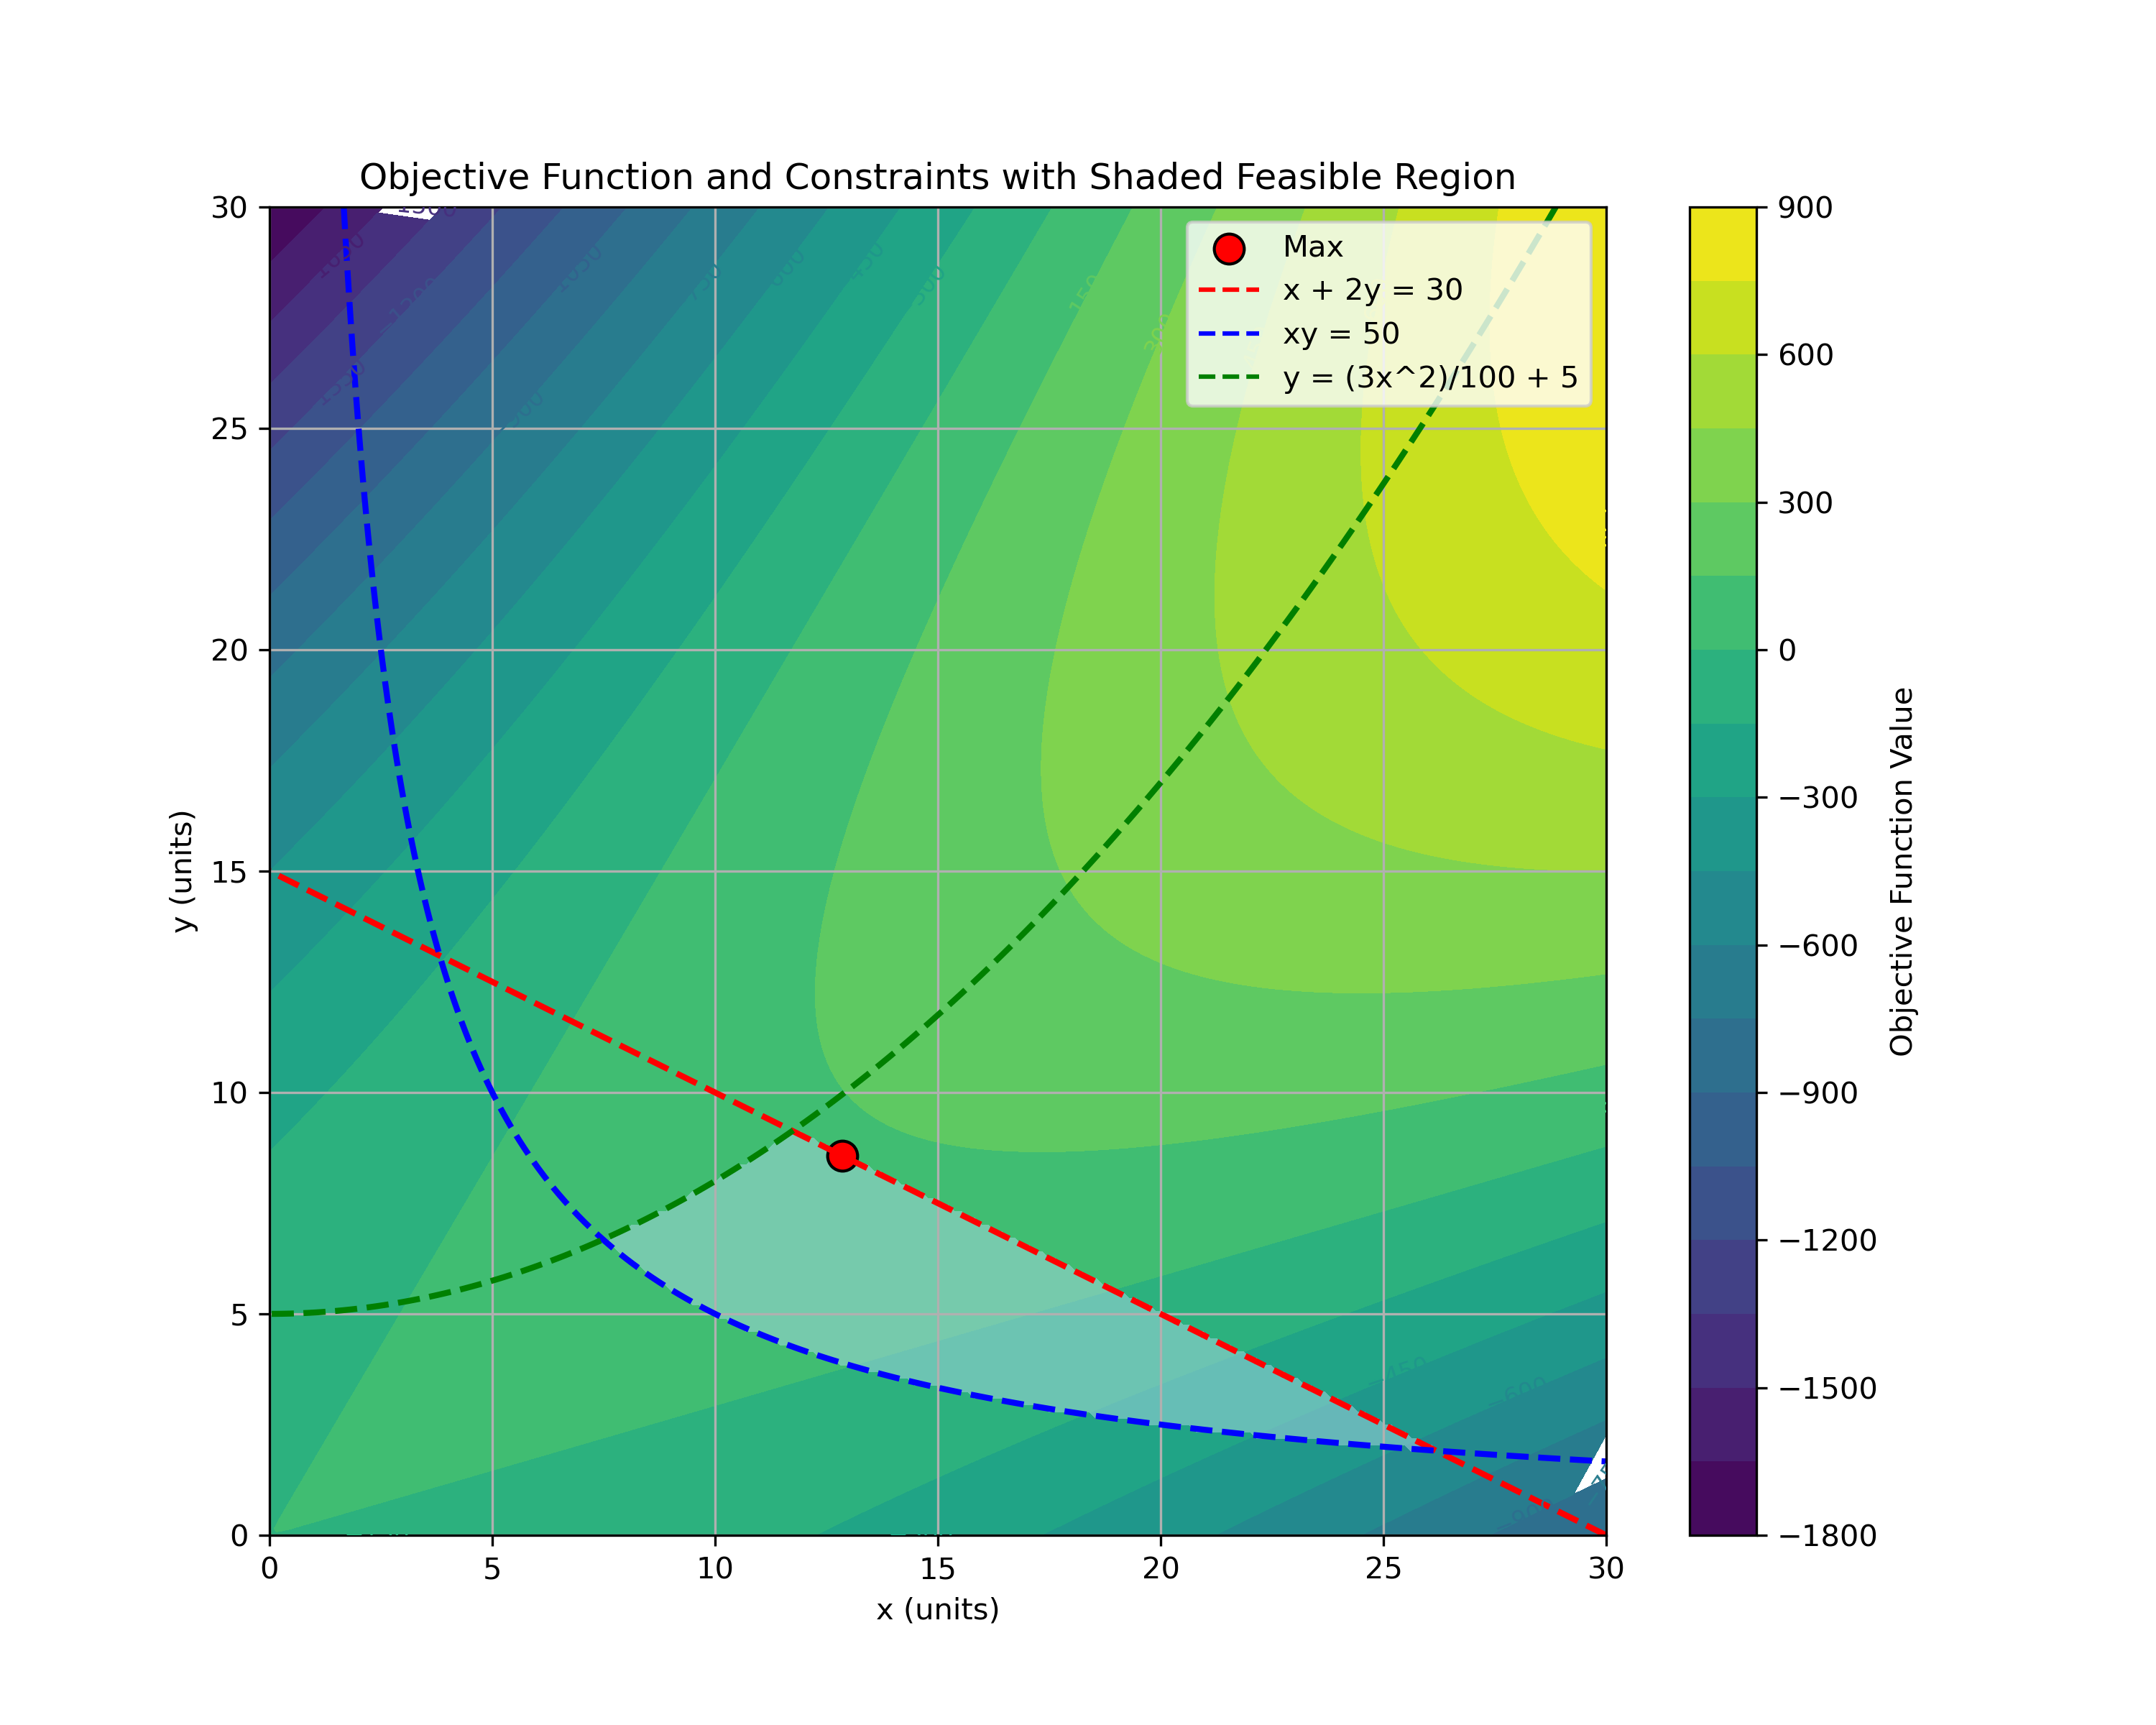
\includegraphics[scale=0.7]{NLO2.png}
        \captionof{figure}{Contour plot of the objective function \( f(x, y) = -x^2 + 4xy - 2y^2 \) with constraints \(x + 2y \leq 30\) (red dashed), \(xy \geq 50\) (blue dashed), and \(y \leq \frac{3x^2}{100} + 5\) (green dashed). The light blue region represents the feasible area where all constraints are satisfied. The solution obtained with \autoref{code:NLO2}}
    \label{Fig:NLO2}
\end{minipage}

\blacksquare
\Exercise Optimization of $f(x, y) = x^2 - y$ subject to $x^2 + y^2 = 4$

\Answer 

We will use the method of Lagrange multipliers.

{\bf Step 1: Define the Lagrange Function}
Define the constraint as $g(x, y) = x^2 + y^2 - 4 = 0$. The Lagrange function is then:
\[
\mathcal{L}(x, y, \lambda) = f(x, y) + \lambda \cdot g(x, y) = x^2 - y + \lambda(x^2 + y^2 - 4).
\]

{\bf Step 2: Compute the Partial Derivatives}
We now compute the partial derivatives of $\mathcal{L}(x, y, \lambda)$ with respect to $x$, $y$, and $\lambda$:

\begin{align*}
\frac{\partial \mathcal{L}}{\partial x} &= 2x + \lambda \cdot 2x = 2x(1 + \lambda) = 0, \\
\frac{\partial \mathcal{L}}{\partial y} &= -1 + \lambda \cdot 2y = 0 \quad \Rightarrow \quad \lambda = \frac{1}{2y}, \\
\frac{\partial \mathcal{L}}{\partial \lambda} &= x^2 + y^2 - 4 = 0.
\end{align*}

{\bf Step 3: Solve the Equations}

\subparagraph{From $\frac{\partial \mathcal{L}}{\partial x} = 0$:}
\[
2x(1 + \lambda) = 0.
\]
This gives two possibilities:
\begin{itemize}
  \item $x = 0$, or
  \item $1 + \lambda = 0 \quad \Rightarrow \quad \lambda = -1$.
\end{itemize}


\subparagraph{Case 1: $x = 0$}
Substitute $x = 0$ into the constraint equation $x^2 + y^2 = 4$:
\[
0^2 + y^2 = 4 \quad \Rightarrow \quad y^2 = 4 \quad \Rightarrow \quad y = \pm 2.
\]
For $y = 2$, substitute into $f(x, y) = x^2 - y$:
\[
f(0, 2) = 0^2 - 2 = -2.
\]
For $y = -2$, substitute into $f(x, y)$:
\[
f(0, -2) = 0^2 - (-2) = 2.
\]

\subparagraph{Case 2: $\lambda = -1$}
Substitute $\lambda = -1$ into $\lambda = \frac{1}{2y}$:
\[
-1 = \frac{1}{2y} \quad \Rightarrow \quad y = -\frac{1}{2}.
\]
Now, substitute $y = -\frac{1}{2}$ into the constraint equation $x^2 + y^2 = 4$:
\[
x^2 + \left(-\frac{1}{2}\right)^2 = 4 \quad \Rightarrow \quad x^2 + \frac{1}{4} = 4 \quad \Rightarrow \quad x^2 = \frac{15}{4} \quad \Rightarrow \quad x = \pm \frac{\sqrt{15}}{2}.
\]
Now, calculate $f(x, y) = x^2 - y$ for $y = -\frac{1}{2}$ and $x = \pm \frac{\sqrt{15}}{2}$:

For $x = \frac{\sqrt{15}}{2}$:
\[
f\left(\frac{\sqrt{15}}{2}, -\frac{1}{2}\right) = \left(\frac{\sqrt{15}}{2}\right)^2 - \left(-\frac{1}{2}\right) = \frac{15}{4} + \frac{1}{2} = \frac{17}{4}.
\]
For $x = -\frac{\sqrt{15}}{2}$:
\[
f\left(-\frac{\sqrt{15}}{2}, -\frac{1}{2}\right) = \left(-\frac{\sqrt{15}}{2}\right)^2 - \left(-\frac{1}{2}\right) = \frac{15}{4} + \frac{1}{2} = \frac{17}{4}.
\]

{\bf Step 4: Compare the Results}
We now compare the function values:
\begin{itemize}
    \item For $(0, 2)$: $f(0, 2) = -2$.
    \item For $(0, -2)$: $f(0, -2) = 2$.
    \item For $\left(\frac{\sqrt{15}}{2}, -\frac{1}{2}\right)$ and $\left(-\frac{\sqrt{15}}{2}, -\frac{1}{2}\right)$: $f = \frac{17}{4} \approx 4.25$.
\end{itemize}

{\bf Conclusion}
\begin{itemize}
    \item The maximum value is $f = \frac{17}{4} \approx 4.25$ at $\left(\frac{\sqrt{15}}{2}, -\frac{1}{2}\right)$ and $\left(-\frac{\sqrt{15}}{2}, -\frac{1}{2}\right)$.
    \item The minimum value is $f = -2$ at $(0, 2)$.
\end{itemize}

For a Python implementation check \href{https://github.com/Biocomputing-Teaching/ORcourse/blob/main/code/lagrange.py}{this file}.

\Exercise Maximize $f(x,y)=xy$ subject to $100 \geq x+y$ and $x\leq 40$ and $(x,y)\geq0$.

\Answer 

The Karush Kuhn Tucker (KKT) conditions  for optimality are a set of necessary conditions for a solution to be optimal in a mathematical optimization problem. They are necessary and sufficient conditions for a local minimum in nonlinear programming problems. The KKT conditions consist of the following elements:

For an optimization problem in its standard form:

\begin{equation*}
  \begin{aligned}
    \text{max} \, f(\uvec{x}) \\
    \text{s.t.}\quad &
    \begin{array}{rcl}
      g_i(\uvec{x})-b_i  & \leq & 0 \quad i=1,\ldots,k \\
      g_i(\uvec{x})-b_i  & = & 0 \quad i=k+1,\ldots,m \\
    \end{array}
  \end{aligned}
\end{equation*}

There are 4 KKT conditions for optimal primal ($\uvec{x}$) and dual ($\lambda$) variables. If $\uvec{x}^*$ denotes optimal values:
\begin{enumerate}
  \item Primal feasibility: all constraints must be satisfied: $g_i(\uvec{x}^*)-b_i$ is feasible. Applies to both equality and non-equality constraints.
  \item Gradient condition or No feasible descent: No possible improvement at the solution: 
  \[ \nabla f(\uvec{x}^*)-\sum_{i=1}^m \lambda_i^* \nabla g_i (\uvec{x}^*)=0\]
  \item Complementariety slackness: 
  \[\lambda_i^* (g_i(\uvec{x}^*)-b_i)=0\]
  \item Dual feasibility: $\lambda_i^*\geq 0$
\end{enumerate}

The last two conditions (3 and 4) are only required with inequality constraints and enforce a positive Lagrange multiplier when the constraint is active (=0) and a zero Lagrange multiplier when the constraint is inactive (>0). 

To solve our problem, first we will put it in its standard form:


\begin{equation}
  \begin{aligned}
    \text{max} \, f(x,y)=xy \\
    \text{s.t.}\quad &
    \begin{array}{rcl}
      g_1(x,y)=x+y-100  & \leq & 0  \\
      g_2(x,y)=x-40 & \leq & 0  \\
      g_3(x,y)=-x&\leq&0\\
      g_4(x,y)=-y&\leq&0\\
    \end{array}
  \end{aligned}
  \label{Eq:KKT}
\end{equation}

\begin{minipage}[t]{\linewidth}
  \vspace{-2ex}
\begin{center}
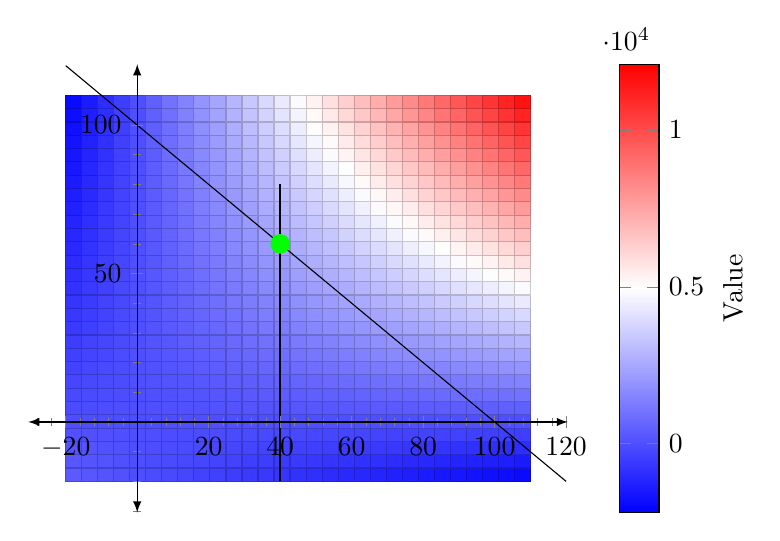
\begin{tikzpicture}
  \begin{axis}
    [ 
      xmin=-30, xmax=120,
      ymin=-30, ymax=120,
      grid=both,
      grid style={line width=.1pt, draw=darkgray!10},
      major grid style={line width=.2pt, draw=darkgray!50},
      axis lines=middle,
      minor tick num=4,
      enlargelimits={abs=0.5},
      axis line style={latex-latex},
      samples=30,
      domain=-20:110,
      view={0}{90},
      % Set contour options
      colormap={blueyellow}{color=(blue) color=(white) color=(red)},
      colorbar,
      colorbar style={ylabel={Value}}
    ]

    % Fill area under the blue region
    \fill[blue, pattern=north west lines, pattern color=blue] (0,0) -- (0,100) -- (40,60) -- (40,0) -- (0,0);
    
    
    % Add surface plot for z = x * y
    \addplot3 [surf, samples=30, domain=-20:110] {x*y}; % Create the surface plot

    % Draw lines
    \draw[black, thick] (40,-20) -- (40,80);
    \draw[black] (-20,120) -- (120,-20);

    \node at (40,60)[circle,fill,green,inner sep=2.5pt]{};

  \end{axis}
\end{tikzpicture}
\end{center}
\captionof{figure}{Contour plot of the objective function \( f(x, y) = xy \) with constraints in Eq. \ref{Eq:KKT}, showing the final optimal value after applying the KKT conditions (green dot).}
\label{Fig:KKT}
\end{minipage}

We will go through the different conditions:

 \begin{itemize}
  \item on the gradient:
  \[
    \begin{pmatrix}\pdv{f}{x}\\\pdv{f}{y}\end{pmatrix} 
    -\lambda_1 \begin{pmatrix}\pdv{g_1}{x}\\\pdv{g_1}{y}\end{pmatrix}
    -\lambda_2 \begin{pmatrix}\pdv{g_2}{x}\\\pdv{g_2}{y}\end{pmatrix} 
    -\lambda_3 \begin{pmatrix}\pdv{g_3}{x}\\\pdv{g_3}{y}\end{pmatrix}
    -\lambda_4 \begin{pmatrix}\pdv{g_4}{x}\\\pdv{g_4}{y}\end{pmatrix}=0
  \]
  which, in this example, resolves into:
  \begin{equation}\label{Eq:KKT1}y-(\lambda_1+\lambda_2-\lambda_3)=0\end{equation}
  \begin{equation}\label{Eq:KKT2}x-(\lambda_1-\lambda_4)=0\end{equation}
  \item on the complementary slackness:
  \begin{equation}\label{Eq:KKT3}\lambda_1 (x +y -100)=0\end{equation}
  \begin{equation}\label{Eq:KKT4}\lambda_2 (x-40)=0\end{equation}
  \begin{equation}\label{Eq:KKT5}\lambda_3 x =0\end{equation}
  \begin{equation}\label{Eq:KKT6}\lambda_4 y =0\end{equation}
  \item on the constraints:
  \begin{equation}\label{Eq:KKT7}x+ y \leq100\end{equation}
  \begin{equation}\label{Eq:KKT8}x\leq40\end{equation}
  \begin{equation}\label{Eq:KKT9}-x\leq0\end{equation}
  \begin{equation}\label{Eq:KKT10}-y\leq0\end{equation}

  plus $\lambda_1,\lambda_2,\lambda_3,\lambda_4\geq 0$.

  We will start by checking Eq. \ref{Eq:KKT3}:
  \begin{itemize}
    \item  Let us see what occurs if $\lambda_1=0$. Then, from Eq. \ref{Eq:KKT2}, $x+\lambda_4=0$ which implies that $x=\lambda_4=0$\footnote{Recall that both variables and multiplieras must be positive or zero, so, the only possibility for the equation to fullfill is that both are zero.}. But, then, from Eq. \ref{Eq:KKT4} we obtain that $\lambda_2=0$ which, using Eq. \ref{Eq:KKT1} gives $y+\lambda_3=0\Rightarrow y=\lambda_3=0$. Indeed, the KKT conditions are satisfied when all variables and multipliers are zero, but it is not a maximum of the function (see figure above).
    \item So, let us see what happens if $x+y-100=0$ and consider the two possibilities for $x$:
    \begin{description}
      \item[Case $x=0$:] Then, $y=100$, which would lead (Eq. \ref{Eq:KKT6}) to $\lambda_4=0$ and (Eq. \ref{Eq:KKT2}) to $x=\lambda_1=0$, that was discussed in the previous item. So, we need top explore the other possibility for $x$.
      \item[Case $x>0$:] From Eq. \ref{Eq:KKT5} $\lambda_3=0$ and, from Eqs. \ref{Eq:KKT1} and \ref{Eq:KKT2}:
      \[\systeme{y=\lambda_1+\lambda_2,x=\lambda_1+\lambda_4}
      \] 
      let us try what happens if, e.g., $\lambda_2\neq 0$ (or, said in other words, if constraint \ref{Eq:KKT8} is active): $x=40$. As we know we do not want $\lambda_1=0$, from Eq. \ref{Eq:KKT3} we obtain $x+y-100=0\Rightarrow y=60$.
    \end{description}

    The point $(x,y)=(40,60)$ fullfills the KKT conditions and is a maximum in the constrained maximization problem (as can be seen in \autoref{Fig:KKT}).

 \end{itemize}
\end{itemize}

\section{Duality}
\Exercise Consider the linear programming problem:
\begin{equation*}
  \begin{aligned}
    \text{max} \, x_1+4x_2+2x_3 \\
    \text{s.t.}\quad &
    \begin{array}{rcl}
      5x_1+2x_2+2x_3  & \leq & 145 \\
      4x_1+8x_2-8x_3  & \leq & 260 \\
      x_1+x_2+4x_3  & \leq & 190 \\
      x_1,x_2x_3  & \geq & 0 \\
    \end{array}
  \end{aligned}
\end{equation*}
Find $x_1$, $x_2$ and $x_3$ to solve it.

\Answer 

material: complementary slackness.pdf
\Exercise Consider the linear programming problem:
\begin{equation*}
  \begin{aligned}
    \text{max} \, 2x_1 + 16x_2 + 2x_3 \\
    \text{s.t.}\quad &
    \begin{array}{rcl}
      2x_1 + x_2-x_3  & \leq & -3 \\
      -3x_1+x_2+2x_3& \leq & 12 \\
      x_1,x_2x_3  & \geq & 0 \\
    \end{array}
  \end{aligned}
\end{equation*}
Check whether each of the following is an optimal solution, using complementary slackness:

\Answer 

material: compslack.pdf

\section{Network analysis}
\Exercise The figure shows a network on four nodes, including net demands on the vertex, $b_k$, and cost an capacity on the edges, $(c_{i,j},u_{i,j})$.(Adapted from \cite{rardin2017}) 

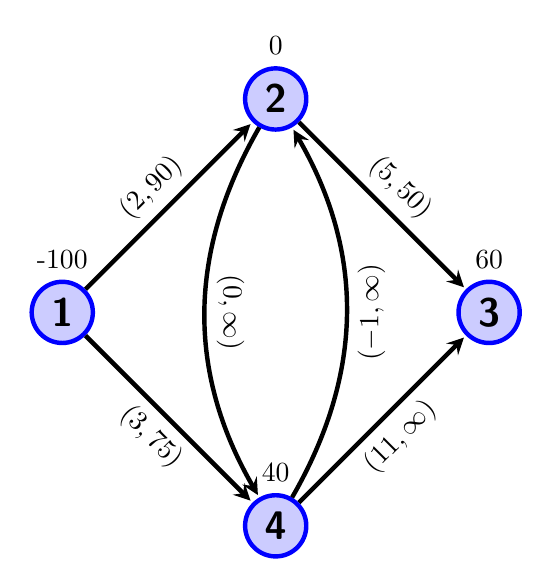
\begin{tikzpicture}[shorten >=1pt, auto, node distance=3cm, ultra thick,
  node_style/.style={circle,draw=blue,fill=blue!20!,font=\sffamily\Large\bfseries},
  edge_style/.style={draw=black, ultra thick},
  arrow_style/.style={draw=black, ultra thick,-stealth},
  every edge quotes/.append style = {anchor=north, sloped}],
                      
  \node (v1) [node_style, label=-100] {1};
  \node (v2) [node_style, label=0, above right=of v1] {2};
  \node (v3) [node_style, label=60, below right=of v2] {3};
  \node (v4) [node_style, label=40, below right=of v1] {4};
  %
  \draw [arrow_style] (v1) edge node[above,sloped]{$(2,90)$} (v2);
  \draw [arrow_style] (v1) edge node[below,sloped]{$(3,75)$} (v4);
  \draw [arrow_style,bend right] (v4) edge node[below,sloped]{$(-1,\infty)$} (v2);
  \draw [arrow_style,bend right] (v2) edge node[above,sloped]{$(0,\infty)$} (v4); 
  \draw [arrow_style] (v2) edge node[above,sloped]{$(5,50)$} (v3);    
  \draw [arrow_style] (v4) edge node[below,sloped]{$(11,\infty)$} (v3); 
      \end{tikzpicture}

\begin{enumerate}
  \item Formulate the corresponding minimum cost network flow model
  \item Classify the nodes as {\em source}, {\em sink} or {\em transshipment}
\end{enumerate}

\Answer 

In this  problem, vertex and edges are:
\begin{eqnarray*}
  V&=&\{1,2,3,4\}\\
  A&=&\{(1,2),(1,4),(2,3),(2,4),(4,2),(4,3)\}
\end{eqnarray*}

we can use the variables $x_{i,j}$ to represent the flows in the different members of set $A$. Thus, the formulation of the problem is:
\begin{equation*}
  \begin{aligned}
    \text{min} \quad&2x_{1,2}+3x_{1,4}+5x_{2,3}-x_{4,2}+11x_{4,3} \\
    \text{subject to }\quad &
    \syssubstitute{A{x_{1,2}}B{x_{1,4}}C{x_{2,3}}D{x_{2,4}}E{x_{4,3}}F{x_{4,2}}}
\systeme[ABCDEF]{
  -A-B=-100,
  A+F-C-D=0,
  C+E=60,
  B+D-F-E=40,
  A\leq 90,
  B\leq 75,
  C\leq 50} 
\end{aligned}\\
\end{equation*}
and $x_{i,j}\geq 0$.

There are 4 KKT conditions for optimal primal ($x4$) and dual ($\lambda$) variables. If $x^*$ denotes optimal values:
\begin{enumerate}
  \item Primal feasibility: all constraints must be satisfied: $g_i(x^*)-b_i$ is feasible. Applies to both equality and non-equality constraints.
  \item Gradient condition or No feasible descent: No possible improvement at the solution: 
  \[ \nabla f(x^*)-\sum_{i=1}^m \lambda_i^* \nabla g_i (x^*)=0\]
  \item Complementariety slackness: 
  \[\lambda_i^* (g_i(x^*)-b_i)=0\]
  \item Dual feasibility: $\lambda_i^*\geq 0$
\end{enumerate}

The last two conditions (3 and 4) are only required with inequality constraints and enforce a positive Lagrange multiplier when the constraint is active (=0) and a zero Lagrange multiplier when the constraint is inactive (>0). 

to solve our problem, first we will put it in its standard form:


\begin{equation*}
  \begin{aligned}
    \text{min } f(x,y)=-xy \\
    \text{subject to }\quad &
    \begin{array}{rcl}
      -x-y+100  & \geq & 0  \\
      -x-40 & \geq & 0  \\
    \end{array}
  \end{aligned}
\end{equation*}

We will go through the different conditions:

\begin{enumerate}
  \item Primal feasibility:  $g_i(x^*)-b_i$ is feasible. 
  \[-x^* -y^* +100 =0\]
  \[-x^*-40=0\]
  \item Gradient condition or No feasible descent:  
  \[ \begin{pmatrix}\pdv{f}{x}\\\pdv{f}{y}\end{pmatrix} 
  -\lambda_1 \begin{pmatrix}\pdv{g_1}{x}\\\pdv{g_1}{y}\end{pmatrix}
  -\lambda_2 \begin{pmatrix}\pdv{g_2}{x}\\\pdv{g_2}{y}\end{pmatrix} =0\]
  which, in this example, resolves into:
  \[\systeme[xy\lambda_1\lambda_2]{-y+\lambda_1+\lambda_2=0,-x-\lambda_1=0 }\]
  \item Complementariety slackness: 
  \[\lambda_1^* (-x^* -y^* +100)=0\]
  \[\lambda_2^* (-x^*-40)=0\]
  \item Dual feasibility: $\lambda_1,\lambda_2\geq 0$
\end{enumerate}

We can put the resulting 5 expressions for conditions 1 and 2 into matrix form:

\[
  \begin{pmatrix} -1 & -1 & 0&0\\ -1&0&0&0\\ 0&-1&1&1\\ -1&0&-1&0 \end{pmatrix}
  \begin{pmatrix} x\\y\\\lambda_1\\\lambda_2\end{pmatrix}=
  \begin{pmatrix} -100\\ 40\\0\\0 \end{pmatrix}
\]

  % \begin{minipage}[t]{\linewidth}
  %   \vspace{-2ex}
  %   %\includegraphics[width=\textwidth]{../figures/Afiquadrilater.pdf}
  %   \captionof{figure}{Transformacions afins d'un quadrilàter de vèrtex $(4,0)$, $(2,2)$, $(1,1)$ i $(2,-1)$.}
  %   \label{fig:trafquadril}
  % \end{minipage}

\end{ExerciseList}

\section{Appendices}

\subsection{Python codes}

\lstlistoflistings

\subsubsection{NLO with constraints}

\pythonexternal[caption=Non-linear optimization with constraints,label=code:NLO2]{../code/NLO2solution.py}

% \tcbinputlisting{%
%    arc=0pt, 
%    outer arc=0pt,
%    listing only,
%    colback=blue!10,
%    colbacktitle=blue!75!black,
%    listing style=Matlab-editor,
%    title=Accuracy Calculation,
%    hbox,
%    enhanced,
%    drop shadow,
%    listing file=../code/NLO2solution.py
% }

\bibliographystyle{plain}
\bibliography{refs}

\end{document}